\documentclass[a4paper]{article}

\usepackage[utf8]{inputenc}
\PassOptionsToPackage{hyphens}{url} % zodat url's ook afgekapt worden
\usepackage{hyperref}
\usepackage[dutch]{babel}
\usepackage{graphicx}
\usepackage{algorithm}
\usepackage{algorithmic}
\usepackage{mathtools}
\usepackage{tikz}
\usepackage{tocbibind}
\usepackage{float}
\usepackage{framed}
\usepackage{parskip}
\usepackage{listings}
\usepackage{color}
\usepackage{pdfpages}
\usepackage{pdflscape}
\usepackage{todonotes}

\title{Software Engineering Analyse: \\ Deeltijds Onderwijs Management Systeem}
\author{Vincent Drozdzyniak 1334231 \\ Hendrik Lievens 1130921 \\ Martijn Maes 1131102 \\ Reinaert Van de Cruys 1334947 \\ Michiel Vanmunster 1334724 \\ Jens Vannitsen 1334039}
\date{3 maart 2016}

\begin{document}
\maketitle



\section{Probleemstelling}
Steven Vandormael, leerkracht bij Centrum voor Deeltijds Onderwijs Technisch Instituur Heilig Hart, draagt ons een project op waarin een rapportensysteem moet worden ontwikkeld voor het deeltijds onderwijs. Voor het secundair onderwijs bestaan reeds verschillende rapportensystemen, denk maar aan Smartschool. Zulke systemen zijn echter niet geschikt voor het deeltijds onderwijs, omdat dit erg verschillend is van het secundair onderwijs.

In het deeltijds onderwijs gaan jongeren deeltijds naar school, en deeltijds werken in een bedrijf. Ze krijgen wekelijks 7 uur project algemene vakken (PAV), en 8 uur beroepsgerichte vorming (BGV). Het doel van PAV is dat de leerling verschillende competenties uit het leerplan verwerft. Bij BGV kan de leerling een certificaat verwerven voor het specifieke beroep waar hij/zij een opleiding voor volgt. Dit is het voornaamste verschil met het secundair onderwijs, wat puntengeoriënteerd is (taken, toetsen, ...).

Het rapportensysteem moet een overzichtelijk rapport kunnen voorleggen aan de leerling en diens ouders.\\
PAV leerkrachten moeten projecten kunnen aanmaken waaraan competenties gekoppeld zijn. Per competentie kan de leerkracht een score toekennen aan de leerlingen en er commentaar bijvoegen.\\
BGV leerkrachten moeten een score kunnen toekennen aan de competenties van een deelcerticaat, binnen het certificaat dat de leerling tracht te behalen.\\

\newpage

\section{Requirements analyse} 
De functionele requirements zijn:
\begin{enumerate}
% algemeen
\item Het systeem moet toelaten om gebruikers toe te voegen en te verwijderen.
\item Het systeem moet toelaten om aan een gebruiker een rol (leerkracht, leerling, admin) toe te kennen.
\item Het systeem moet toelaten om in te stellen of een leerling al dan niet actief is.
\item Het systeem moet toelaten om de persoonlijke informatie van een leerling aan te passen.
\item De admin moet meldingen ontvangen wanneer een leerling zijn persoonlijke informatie gewijzigd heeft.
\item Het systeem moet toelaten om inschrijvingsgeralteerde informatie van een leerling aan te passen.
\item Het systeem moet toelaten om informatie over de leerkrachten te bewerken.
\item Het systeem moet toelaten om graden toe te voegen, te verwijderen en te bewerken.
\item Het systeem moet toelaten om klassen/richtingen toe te voegen, te verwijderen en te bewerken.
\item Het systeem moet toelaten om subklassen aan een klas/richting toe te voegen, te verwijderen en te bewerken.  % klas voor in de voormiddag, klas voor in de namiddag
\item Het systeem moet toelaten om leerlingen aan een subklas toe te voegen en te verwijderen.
% PAV
\item Het systeem moet toelaten om, in het algemeen, PAV-competenties toe te voegen, te verwijderen en te bewerken.
\item Het systeem moet toelaten om projecten/vakthema's binnen een graad te definiëren, op basis van PAV-competenties, ze te verwijderen en aan te passen.
% BGV
\item Het systeem moet toelaten om BGV-certificaten toe te voegen, te verwijderen en te bewerken.
\item Het systeem moet toelaten om deelcertificaten aan een BGV-certificaat toe te voegen, te verwijderen en te bewerken.
% algemeen (scores)
\item Het systeem moet toelaten om een score (A,I,V) toe te kennen aan een competentie binnen een vakthema, voor een leerling.  % PAV
\item Het systeem moet toelaten om een score (A,I,V) toe te kennen aan een competentie binnen een deelcertificaat, voor een leerling.  % BGV
\item Het systeem moet automatisch het behalen van een competentie blokkeren, indien deze reeds drie maal verworven (score V) werd.  % 3x verwerven == behaald
\item Het systeem moet automatisch de datum waarop een competentie verworven werd, weergeven.
\item Het systeem moet toelaten om een beschrijving te geven bij het verwerven van een competentie.
\item Het systeem moet toelaten om een ingevuld rapport te genereren, voor een leerling.
\item Het systeem moet toelaten om statistieken op te vragen per leerling, over zijn/haar behaalde competenties.
\item Het systeem moet toelaten om de houdingen/attitudes van de leerlingen in te vullen.
% algemeen
\item Het systeem moet toelaten om informatie over de school aan te passen.
\item Het systeem moet toelaten om werkgevers waar de school mee samenwerkt toe te voegen en te verwijderen, en hun informatie aan te passen.
\item Het systeem moet toelaten om een werkgever (waar de school mee samenwerkt) aan een leerling toe te wijzen.
\item Het systeem moet toelaten om een contract te genereren voor de samenwerking tussen leerling en werkgever.
\item Het systeem mag toelaten om berichten te versturen naar anderen.  % optioneel dus
\item Het systeem mag toelaten om bestanden te uploaden.  % optioneel dus 
\item Het systeem mag een app voorzien, waarin de functionaliteiten voor leerlingen en leerkrachten beschikbaar zijn.\\  % optioneel dus 
\end{enumerate}


\section{URPS} 
\subsection{Usability}
De UI is een zeer belangrijk onderdeel van dit systeem. Deze moet overzichtelijk, duidelijk, vlot en consistent zijn, kortom gebruiksvriendelijk. Dit moet zowel voor de leerling, leerkracht als admin het geval zijn. Het is ook belangrijk dat dit op ieder platform waarop het systeem gebruikt wordt, het geval is. Daartoe zou aan responsive webdesign kunnen gedaan worden.

\subsection{Reliability}
Het systeem zal uitgebreid gebruik maken van een database, waardoor de reliablilty van ons systeem hiervan afhangt. We zullen zelf geen invloed hebben op de beschikbaarheid van de server, maar wensen deze zo laag mogelijk te hebben. Reliability is belangrijk voor dit systeem.

\subsection{Performance}
Performantiegewijs zijn er geen echte vereisten, zo lang op alle acties een snelle respons komt ($<$ 2 sec.). Op die manier wordt de gebruiksvriendelijkheid niet verminderd. Het systeem moet wel in staat zijn om een grote school, bestaande uit vele leerlingen, te ondersteunen.

\subsection{Supportability}
Het systeem moet makkelijk uitbreidbaar zijn. Zo waren er reeds de suggesties om een berichtenfunctionaliteit en file-uploadfunctionaliteit toe te voegen. Het systeem moet ook eenvoudig onderhoudbaar zijn, in geval van onderwijshervormingen bv.

\subsection{Legal}
Het systeem moet voldoen aan de wetgeving omtrent privacy voor de punten en persoonlijke informatie van de leerlingen.


\section{Kost}
We schatten zo'n 30 dagen per persoon nodig te hebben, dit komt neer op zo'n 180 werkdagen. Dit is exclusief het optionele berichtensysteem en het optionele file-upoadsysteem.

\section{Mockups}
\begin{figure}[H]
\centering
  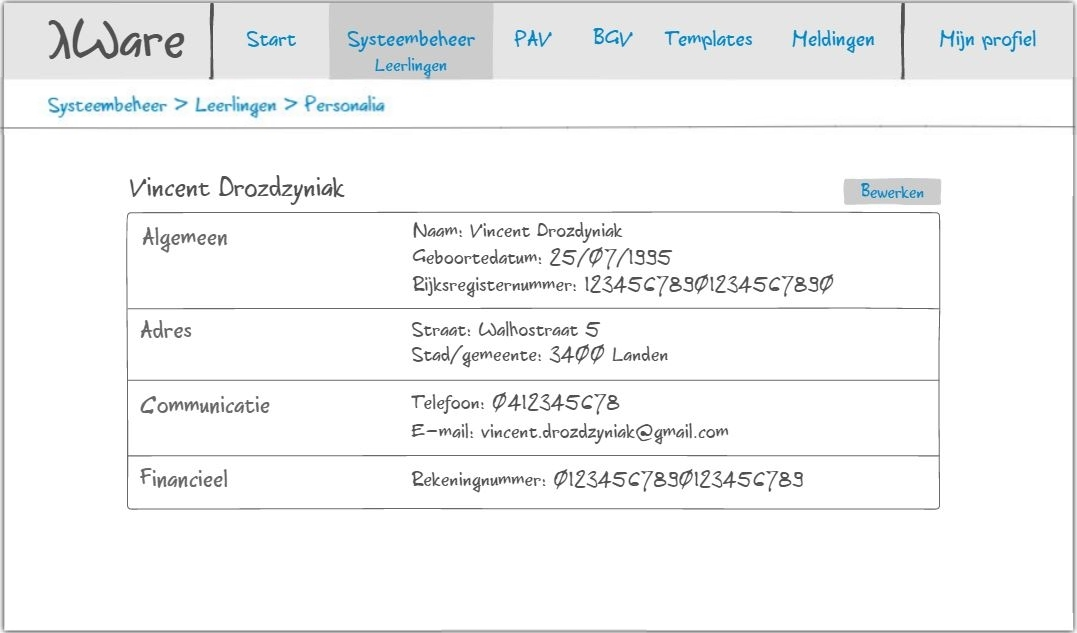
\includegraphics[width=1.0\linewidth]{deeltijdsonderwijs_mockup.JPG}
\end{figure}



\end{document}